% fphw Assignment
% LaTeX Template
% Version 1.0 (27/04/2019)
%
% This template originates from:
% https://www.LaTeXTemplates.com
%
% Authors:
% Class by Felipe Portales-Oliva (f.portales.oliva@gmail.com) with template 
% content and modifications by Vel (vel@LaTeXTemplates.com)
%
% Template (this file) License:
% CC BY-NC-SA 3.0 (http://creativecommons.org/licenses/by-nc-sa/3.0/)
%
%%%%%%%%%%%%%%%%%%%%%%%%%%%%%%%%%%%%%%%%%

%----------------------------------------------------------------------------------------
%	PACKAGES AND OTHER DOCUMENT CONFIGURATIONS
%----------------------------------------------------------------------------------------

\documentclass[
	12pt, % Default font size, values between 10pt-12pt are allowed
	%letterpaper, % Uncomment for US letter paper size
	%spanish, % Uncomment for Spanish
]{fphw}

% Template-specific packages
\usepackage{multicol}
\usepackage[utf8]{inputenc} % Required for inputting international characters
\usepackage[T1]{fontenc} % Output font encoding for international characters
\usepackage{mathpazo} % Use the Palatino font

\usepackage{graphicx} % Required for including images

\usepackage{booktabs} % Required for better horizontal rules in tables

\usepackage{listings} % Required for insertion of code

\usepackage{enumerate} % To modify the enumerate environment

\usepackage{xcolor}

\definecolor{mGreen}{rgb}{0,0.6,0}
\definecolor{mGray}{rgb}{0.5,0.5,0.5}
\definecolor{mPurple}{rgb}{0.58,0,0.82}
\definecolor{backgroundColour}{rgb}{0.95,0.95,0.92}

\lstdefinestyle{CStyle}{
    backgroundcolor=\color{backgroundColour},   
    commentstyle=\color{mGreen},
    keywordstyle=\color{magenta},
    numberstyle=\tiny\color{mGray},
    stringstyle=\color{mPurple},
    basicstyle=\footnotesize,
    breakatwhitespace=false,         
    breaklines=true,                 
    captionpos=b,                
    keepspaces=true,                 
    numbers=left,                    
    numbersep=5pt,                  
    showspaces=false,                
    showstringspaces=false,
    showtabs=false,                  
    tabsize=2,
    language=C
}
%----------------------------------------------------------------------------------------
%	ASSIGNMENT INFORMATION
%----------------------------------------------------------------------------------------

\title{OS 2022 Problem Sheet \#3} % Assignment title

\author{Joshua Law} % Student name

\date{September 29th, 2022} % Due date

\institute{Jacobs University Bremen \\ Bachelor Of Computer Science} % Institute or school name

\class{CO-562 Operating Systems} % Course or class name

\professor{Dr. Jurgen Schonwalder} % Professor or teacher in charge of the assignment

%----------------------------------------------------------------------------------------

\begin{document}

\maketitle % Output the assignment title, created automatically using the information in the custom commands above

%----------------------------------------------------------------------------------------
%	ASSIGNMENT CONTENT
%----------------------------------------------------------------------------------------

\section*{Problem 3.1: \emph{readers / writers problem }}

\begin{problem}
Below are three incorrect solutions of the readers-writers problem. Explain in which situations the solutions fail to work correctly. The solutions use the following common definitions:\end{problem}
\begin{center}
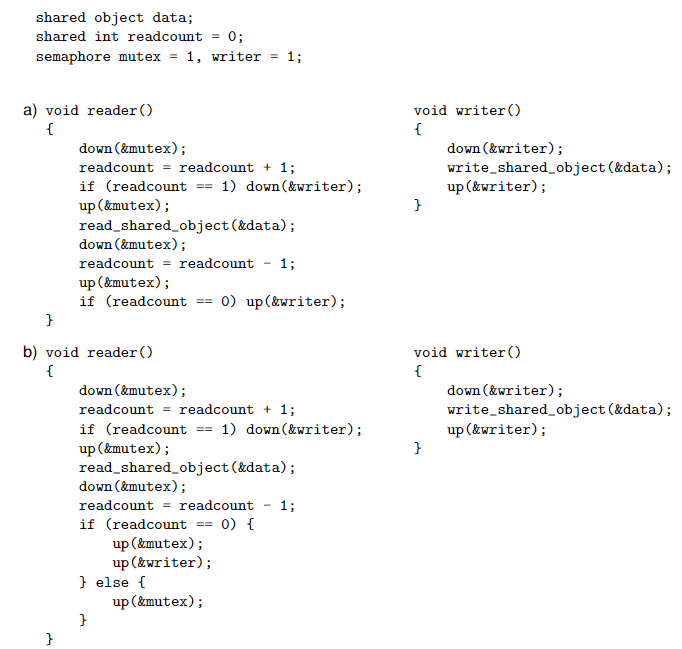
\includegraphics[width=0.8\columnwidth]{Screenshot 2022-09-27 144827.png}
\includegraphics*[width=0.8\columnwidth]{Screenshot 2022-09-27 144929.png}
\end{center}
%------------------------------------------------

\subsection*{Answer}
\begin{enumerate}[\itshape a)\normalfont]
	\item In solution a, at the last if statement, up is used on mutex before the up is used on writer, this creates a concurrency issue where if a writer will be called it would fail as the mutex indicates the process is in use.
	\item In solution b, up is called on mutex before writer during the last if statement so just like solution a a concurrency issue occurs where the mutex indicates it is in use while writer starts its process, which would present the mutex in the wrong state.
	\item In solution c, writer calls down and up on the mutex before and after the writesharedobject, which could mess up the mutex because it is unnecessary for the writer to call the mutex, it might cause an unwanted loop in the mutex state.
\end{enumerate}


%----------------------------------------------------------------------------------------

\section*{Problem 3.2: \emph{perfect numbers (multi threading)}}

\begin{problem}
A perfect number is a positive integer that is equal to the sum of its positive divisors, excluding the
number itself. For example, 6 has the positive divisors \texttt{{ 1, 2, 3 }} and \texttt{1 + 2 + 3 = 6.}
Write a C program called perfect that finds perfect numbers in a range for numbers. The default
number range is \texttt{[1, 10000]}. The program accepts the \texttt{-s} option to set the lower bound and the
\texttt{-e} option to set the higher bound. Hence, the invocation perfect \texttt{-s 100 -e 1000} will search for
perfect numbers in the range \texttt{[100, 1000]}.
The following function can be used to test whether a given number is a perfect number:
\end{problem}
\begin{lstlisting}[style=CStyle]
static int
is_perfect(uint64_t num)
{
	uint64_t i, sum;

	if (num < 2) {
		return 0;
	}
	for (i = 2, sum = 1; i*i <= num; i++) {
		if (num % i == 0) {
			sum += (i*i == num) ? i : i + num / i;
		}
	}
	return (sum == num);
}
\end{lstlisting}	
\begin{enumerate}[\itshape a)\normalfont]
	\item Write a program that searches for perfect numbers in a range of numbers. Your program must support the \texttt{-s} and \texttt{-e} options to define non-default search intervals.\newline \texttt{./perfect -s 100 -e 10000 \newline 496 \newline 8128}

	\item Implement an option \texttt{-t} that can be used to define how many concurrent threads should be used to execute the search. If the \texttt{-t} option is not present, then a single thread is used to carry out the search. For debugging purposes, implement an option \texttt{-v} that writes trace information to the standard error. Below is an invocation with two threads and a verbose trace. \newline \texttt{./perfect -t 2 -v\newline perfect: t0 searching [1,5000] \newline perfect: t1 searching [5001,10000] \newline 6 \newline 28\newline 496\newline 8128\newline perfect: t0 finishing\newline perfect: t1 finishing}
	\item Determine how the \texttt{-t} option impacts the execution time. Pick a search interval that is a reasonable load for your computer hardware and then increase the threading level and determine how the execution time changes. Produce a plot presenting the measurements you have obtained and discuss the results.
\end{enumerate}

	%------------------------------------------------
\subsection*{Answer}

%----------------------------------------------------------------------------------------


\end{document}